\section{Neural Networks as Function Approximators}
\label{ch1:sec3}

In this section we introduce artificial neural networks, usually called neural networks, which are computing systems inspired by the biological neural networks that constitute animal brains. It has been shown that these systems can be used very well as classifiers as well as regressors or function approximators. \\
These neural networks are based on simplified models of biological neurons, which are special cells within the nervous system which transmit information to other nerve cells. Each of these artificial neurons receives data as input. These inputs of one neuron are modified by weights and summed. Finally, an activation function controls the amplitude of the output. The artificial neurons are connected to each other. A single neuron may be connected to many other neurons and the total number of neurons and connections in a network may be extensive. The connections of the biological neuron are modelled as weights, where a positive weight reflects an excitatory connection, while negative values mean inhibitory connections. Each connection, like the synapses in a biological brain, can transmit a signal to other neurons, where the signal is a real number. The other neurons connected to that neuron receive this real number as part of their input and repeat the process. However, artificial neural networks are more about an abstraction of that information processing, less about replicating biological neural networks and neurons. The first mathematical model for a single neuron, termed the perceptron, was described in \cite{Rosenblatt:1958} and is still in use today. We want to use perceptrons and the neural networks constructed from them to generate function values (output) that approximate the values of the solution to our differential equation from data (input) that will be the domain of our differential equation. \\
We now describe how a perceptron transforms a reel-valued input into a one-dimensional output, as illustrated in \cref{fig4}. Let there be $n$ input values $x_1, \ldots, x_n \in \mathbb{R}$, which can be understood as the entries of a vector $x \in \mathbb{R}^n$. First one forms a biased linear combination with the input values, i.e. 
\begin{equation*}
    a = \sum^{n}_{i=1} w_i x_i + b = w^{\mathrm{T}} x + b,
\end{equation*}
where $w_1, \ldots, w_n \in \mathbb{R}$ are called weights and $b \in \mathbb{R}$ is called bias. In general, these weights and the bias are learned through data. Then an activation function $\sigma \colon \mathbb{R} \to \mathbb{R}$, which is non-linear, is applied to the weighted sum $a$, so that the output of the neuron becomes
\begin{equation*}
    z = \sigma(\sum^{n}_{i=1} w_i x_i + b) = \sigma(w^{\mathrm{T}} x + b) = \sigma(a).
\end{equation*}

\begin{figure}[H]
    \begin{center}
        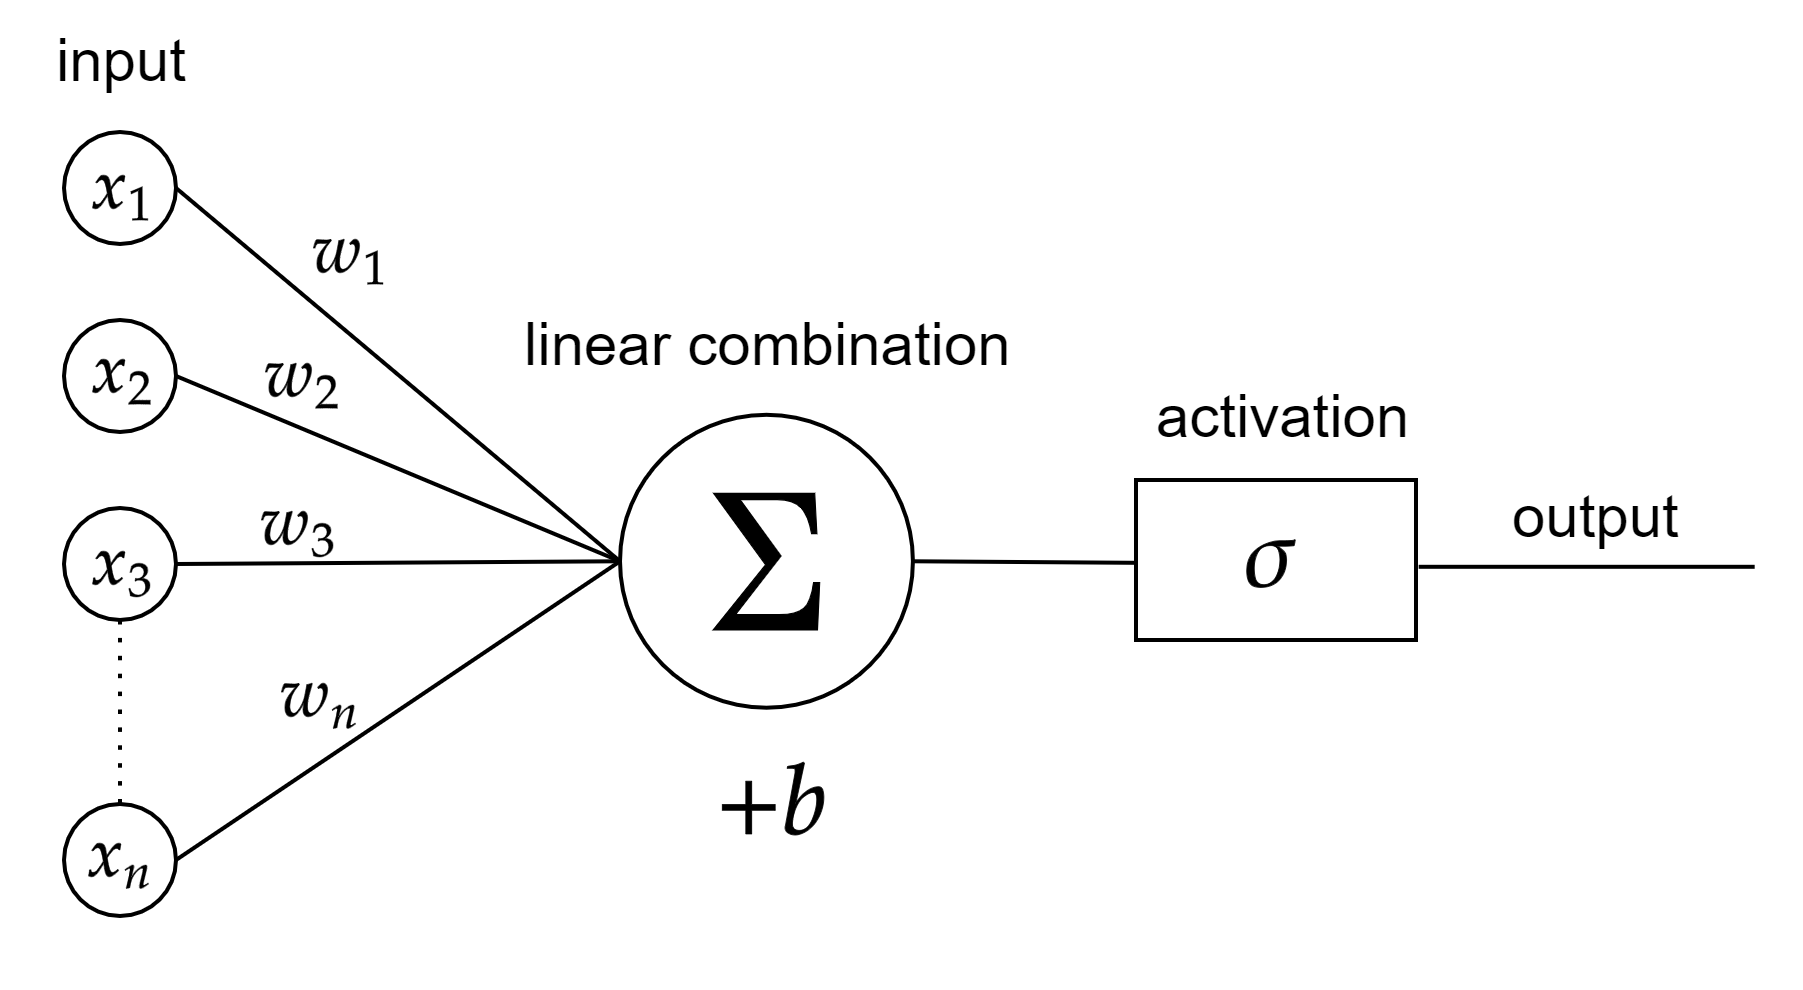
\includegraphics[scale=0.3]{img/diagram-20220205_1.png}
    \end{center}
    \caption{Illustration of the perceptron model for a single neuron.}
    \label{fig4}
\end{figure}

The choice of activation function is determined by the nature of the input and the assumed distribution of the output. When the activation function is for example equal to the Heaviside step function, i.e.
\begin{equation*}
    \sigma(x) = \begin{cases} 1 & \text{if } x \geq 0, \\ 0 & \text{if } x < 0, \end{cases}
\end{equation*}
then the perceptron coincides with a linear support vector classifier, see \cite[Chapter~7]{Bishop:2006}. \\
The activation function can be any non-constant, non-linear function, but those generally used are monotone increasing, continuous, and at least piecewise smooth. At present, the most popular activation function is the rectified linear unit, abbreviated ReLu, \cref{ReLu}. In recent decades, smoother activation functions have been used, such as the sigmoid function, \cref{Sigmoid}, or the hyperbolic tangent function, \cref{TanH}, \cite{}.
\begin{align}
    \sigma(y) &=\max \{y, 0\} & & \text{ rectified linear unit (ReLU) } \label{ReLu} \\
    \sigma(y) &=\frac{1}{1+\exp (-y)} & & \text{ sigmoid } \label{Sigmoid} \\
    \sigma(y) &=\tanh (y)=\frac{\exp (y)-\exp (-y)}{\exp (y)+\exp (-y)} & & \text{ hyperbolic tangent } \label{TanH}
\end{align}
A single perceptron can already be understood as a neural network, but it still has many limitations. Above all, the dimension of the output is limited to $1$. If one wants to create a multi-dimensional output, one arranges several perceptrons in a layer by distributing the input to exactly as many perceptrons as one needs the dimension of the output. Suppose the input has dimension $n$ and the output should have dimension $m$. Then the weights of the $m$ perceptrons are arranged as a matrix $W \in \mathbb{R}^{m \times n}$, where each row corresponds to the $n$ weights of each perceptron, i.e. $w^{i} \in \mathbb{R}^n$ for all $i = 1, \ldots, m$. The biases of the $m$ perceptrons are represented as a vector $b \in \mathbb{R}^m$. The weighted sum of the input $x \in \mathbb{R}^n$ with the addition of a bias for each perceptron can be computed as  
\begin{equation}
    a = W x + b \in \mathbb{R}^m,
\end{equation}
which is also known as the propagation function. 




Frank Rosenblatt showed that a simple perceptron with two input values and a single output neuron can be used to represent the simple logical operators AND, OR and NOT. However, Marvin Minsky and Seymour Papert proved in 1969 that a single-layer perceptron cannot resolve the XOR operator (linear separability problem). This led to a standstill in artificial neural network research.

The inability of a single neuron to model any reasonably complicated function with binary output3
has led to the idea of creating networks of neurons, known as articial neural networks (ANNs).

After mentioning the XOR problem, which cannot be handled by perceptrons with one layer, we introduce multilayer perceptrons. 


Deep-learning methods are representation-learning methods with multiple levels of representation, obtained by composing simple but non-linear modules that each transform the representation at one level (starting with the raw input) into a representation at a higher, slightly more abstract level. With the composition of enough such transformations, very complex functions can be learned.

The most common form of machine learning, deep or not, is supervised learning.

The equations used for computing the forward pass in a neural net



The more complex the problem to be solved with the help of the neural network is, the more layers are needed. 

We compute an objective function that measures the error (or distance) between the output scores and the desired pattern of scores. The machine then modifies its internal adjustable parameters to reduce  this error. These adjustable parameters, often called weights, are real numbers that can be seen as ‘knobs’ that define the input–output function of the machine. In a typical deep-learning system, there may be hundreds of millions of these adjustable weights, and hundreds of millions of labelled examples with which to train the machine. To properly adjust the weight vector, the learning algorithm computes a gradient vector that, for each weight, indicates by what amount the error would increase or decrease if the weight were increased by a tiny amount. The weight vector is then adjusted in the opposite direction to the gradient vector. 

A deep-learning architecture is a multilayer stack of simple modules, all (or most) of which are subject to learning, and many of which compute non-linear input–output mappings. Each module in the stack transforms its input to increase both the selectivity and the invariance of the representation.

The backpropagation procedure to compute the gradient of an objective function with respect to the weights of a multilayer stack of modules is nothing more than a practical application of the chain rule for derivatives. The key insight is that the derivative (or gradient) of the objective with respect to the input of a module can be computed by working backwards from the gradient with respect to the output of that module

Many applications of deep learning use feedforward neural network architectures (Fig. 1), which learn to map a fixed-size input (for example, an image) to a fixed-size output (for example, a probability for each of several categories). To go from one layer to the next, a set of units compute a weighted sum of their inputs from the previous layer and pass the result through a non-linear function. At present, the most popular non-linear function is the rectified linear unit (ReLU), which is simply the half-wave rectifier. In past decades, neural nets used smoother non-linearities, such as , but the ReLU typically learns much faster in networks with many layers, allowing training of a deep supervised network without unsupervised pre-training28. Units that are not in the input or output layer are conventionally called hidden units. The hidden layers can be seen as distorting the input in a non-linear way so that categories become linearly separable by the last layer 


In artificial neural networks, topology refers to the structure of the network. This generally means how many artificial neurons are located on how many layers and how they are connected to each other. Artificial neurons can be connected in many ways to form an artificial neural network. In many models, neurons are arranged in layers one behind the other; 

Perceptron
Activation Function
One layer
Neural Network
FNN
%ResNet
Machine Learning, Training 
Supervised Learning
Unsupervised Learning
Gradient Based optimization
Backpropagation 
Honrik 